\documentclass[12pt]{article}
\usepackage{amssymb}
\usepackage[english]{babel}
\usepackage{fullpage}
\usepackage{graphicx,multirow}
\usepackage{caption}
\usepackage[margin=1.52in]{geometry}
\captionsetup{font=bf,belowskip=11pt}
\usepackage{hyperref}
\usepackage{amsmath}
\usepackage{enumitem}
\usepackage{subfig}
\usepackage{placeins}
\usepackage{tabularray}
\usepackage{float}


\begin{document}
\begin{titlepage} 
	\newcommand{\HRule}{\rule{\linewidth}{0.5mm}}
	\center
	\textsc{\LARGE Polytechnique Montréal}\\[1.5cm]
	\textsc{\Large LOG8415 : Lab B}\\[0.5cm]
	\textsc{\large Advanced Concepts in Cloud Computing}\\[0.5cm]
	\HRule\\[0.4cm]
	{\huge\bfseries MapReduce with Hadoop on AWS (or Azure)}\\[0.4cm]
	\HRule\\[1.5cm]
	{\large\textit{Authors}}\\
	Anis \textsc{Zouatene} (1963304)\\
	Aleksandar \textsc{Stijelja} (1959772)\\
	Amin \textsc{Ghadesi} (2121658)\\
    Reza \textsc{Rouhghalandari} (2153395)\\
	\vfill\vfill\vfill {\large\today} \vfill\vfill
	
\includegraphics{images/poly-logo.png}\\[1cm]
	\vfill
\end{titlepage}


\section{Abstract}

\noindent The programming model known as “MapReduce” facilitates concurrent processing by splitting petabytes of data into smaller chunks and processing them in parallel on Hadoop commodity servers. In the end, it aggregates all the data from multiple servers to return a consolidated output back to the application. \\
\noindent However, we have different ways to manage Big Data sets, such as Apache Hadoop or Apache Spark. In this paper, we will explore both software, compare their differences and evaluate their performances by conducting a few experiments.

\paragraph{Keywords:}Big Data, Azure, MapReduce, Spark, Hadoop, Big Data.

\pagebreak

\section{Introduction} \label{sec:introduction}
\noindent As such, in this lab, we compared the performance of the algorithm on Linux, Hadoop, and Spark with different experiments. We began by comparing  their performances in a simple WordCount program and noted their differences. The WordCount program counts the occurrence of every single word in the specified document. To do this, we chose to use Azure instead of AWS. We then created a VM in it, then we used Hadoop and MapReduce to solve a social networking problem and process bigger data sets. \\
	
\noindent In this lab, we will be presenting the experiments done with the WordCount program, the performance comparison of Hadoop vs. Linux, the performance comparison of Hadoop vs. Spark on Azure, and the “people you might” know algorithm problem. In addition, we explain precisely each step we took for performing this assignment on the GitHub page.  

\bigskip

\pagebreak
	
\section{Experiments with WordCount program}

\noindent Before getting into the performance experiments amongst Hadoop, Spark, and Linux, we began by experimenting with the WordCount program java example given with both Hadoop and Spark. After installing the required Java packages and setting up all environment variables required, we proceeded to run the WordCount example on a copy of pg4300.txt. We made use of the TIME command to be able to extract the time performance of the run. It would provide us with the “real”, “user”, and “sys” duration of the command executed. 

\begin{itemize}
  \item \textbf{real} or \textbf{total} or \textbf{elapsed}: It is the time from start to finish of the command. In other words, it is the time from the moment we hit the Enter key until the moment  the command is completed.
    \item \textbf{user}: The amount of CPU time spent in the user mode.
    \item \textbf{system} or \textbf{sys}: The amount of CPU time spent in the kernel mode.
\end{itemize}

\begin{figure}[!ht]
    \centering
    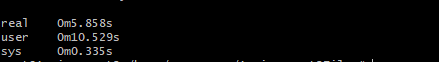
\includegraphics[width=140mm, scale=1.0]{images/hadoop-time.png}
    \caption{The time consumption of Hadoop WordCount.java on pg3000.txt}
    \label{fig:fig1}
\end{figure}

\noindent We have to mention that we utilize real metric for our experiments and result figures. However, it seems we have to use the sum of user and sys times instead of the real time.

\begin{figure}[H]
    \centering
    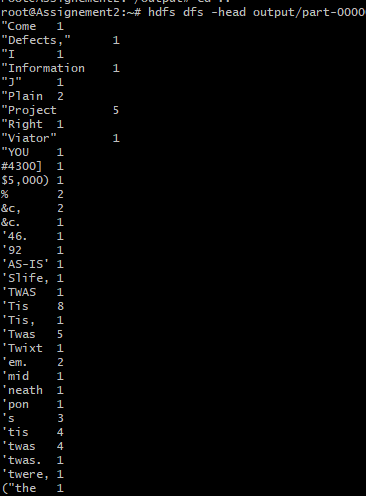
\includegraphics[width=80mm, scale=1.0]{images/output-pg4300.png}
    \caption{Result of Hadoop WordCount.java on pg3000.txt}
    \label{fig:fig2}
\end{figure}

\noindent Figure~\ref{fig:fig1} and \ref{fig:fig2} illustrate the time and the output of Hadoop WordCount.java on pg3000.txt, respectively.

\newpage

\section{Performance comparison of Hadoop vs. Linux}

\noindent Now that we experimented using Hadoop with the word count example talked about previously, we can now start running Hadoop WordCount on all the datasets provided and compare them with Linux. The first step was done in the last section, but for the Linux part, we do not need additional tools except regular pipelining
through command line commands. For implementation, we created an Azure VM where we had to do 3 tests on each to get an average for both.

\begin{figure}[H]
    \centering
    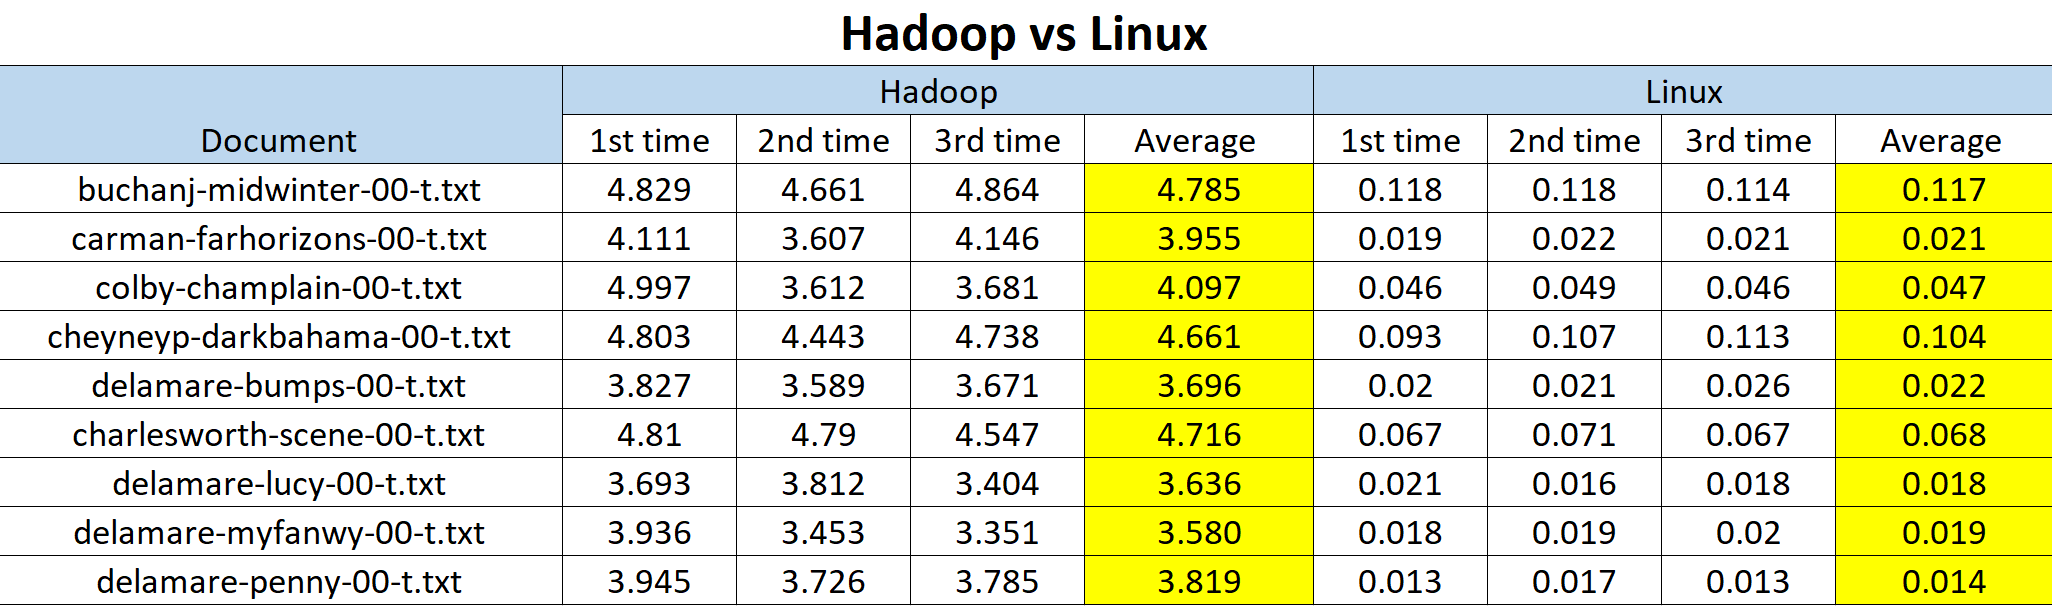
\includegraphics[width=140mm, height=60mm, scale=1.0]{images/Hadoop_vs_Linux_table.PNG}
    \caption{Average run time of Hadoop vs. Linux on each dataset}
    \label{fig:fig3}
\end{figure}

\newpage

\subsection{Results}

\noindent Figure~\ref{fig:fig3} displays the comparison of the consumption time between Hadoop and Linux on each document. Also, for simplicity, we created a bar chart (Figure\ref{fig:fig4}) that shows the average times. We have to mention that all times are in the second unit. By looking at the bar chart, we can see that Linux outperformed Hadoop by a LOT. One of the reasons for this kind of result is that Hadoop needs to take time to convert the input data into HDFS format then proceed with the processing, whereas Linux directly uses the RAM to read the input line by line in order to do the process, cutting off that preparation period that Hadoop needs. This does not mean that Hadoop is inferior, because if we are dealing with large quantities of data, then we expect Hadoop to outperform easily Linux. Technically, in-memory processing is faster as no time is spent in moving the data/processes in and out of the disk, memory and catch. In addition, Hadoop does not suit for small data. (HDFS) Hadoop distributed file system lacks the ability to efficiently support the random reading of small files because of its high capacity design.


\begin{figure}[h]
    \centering
    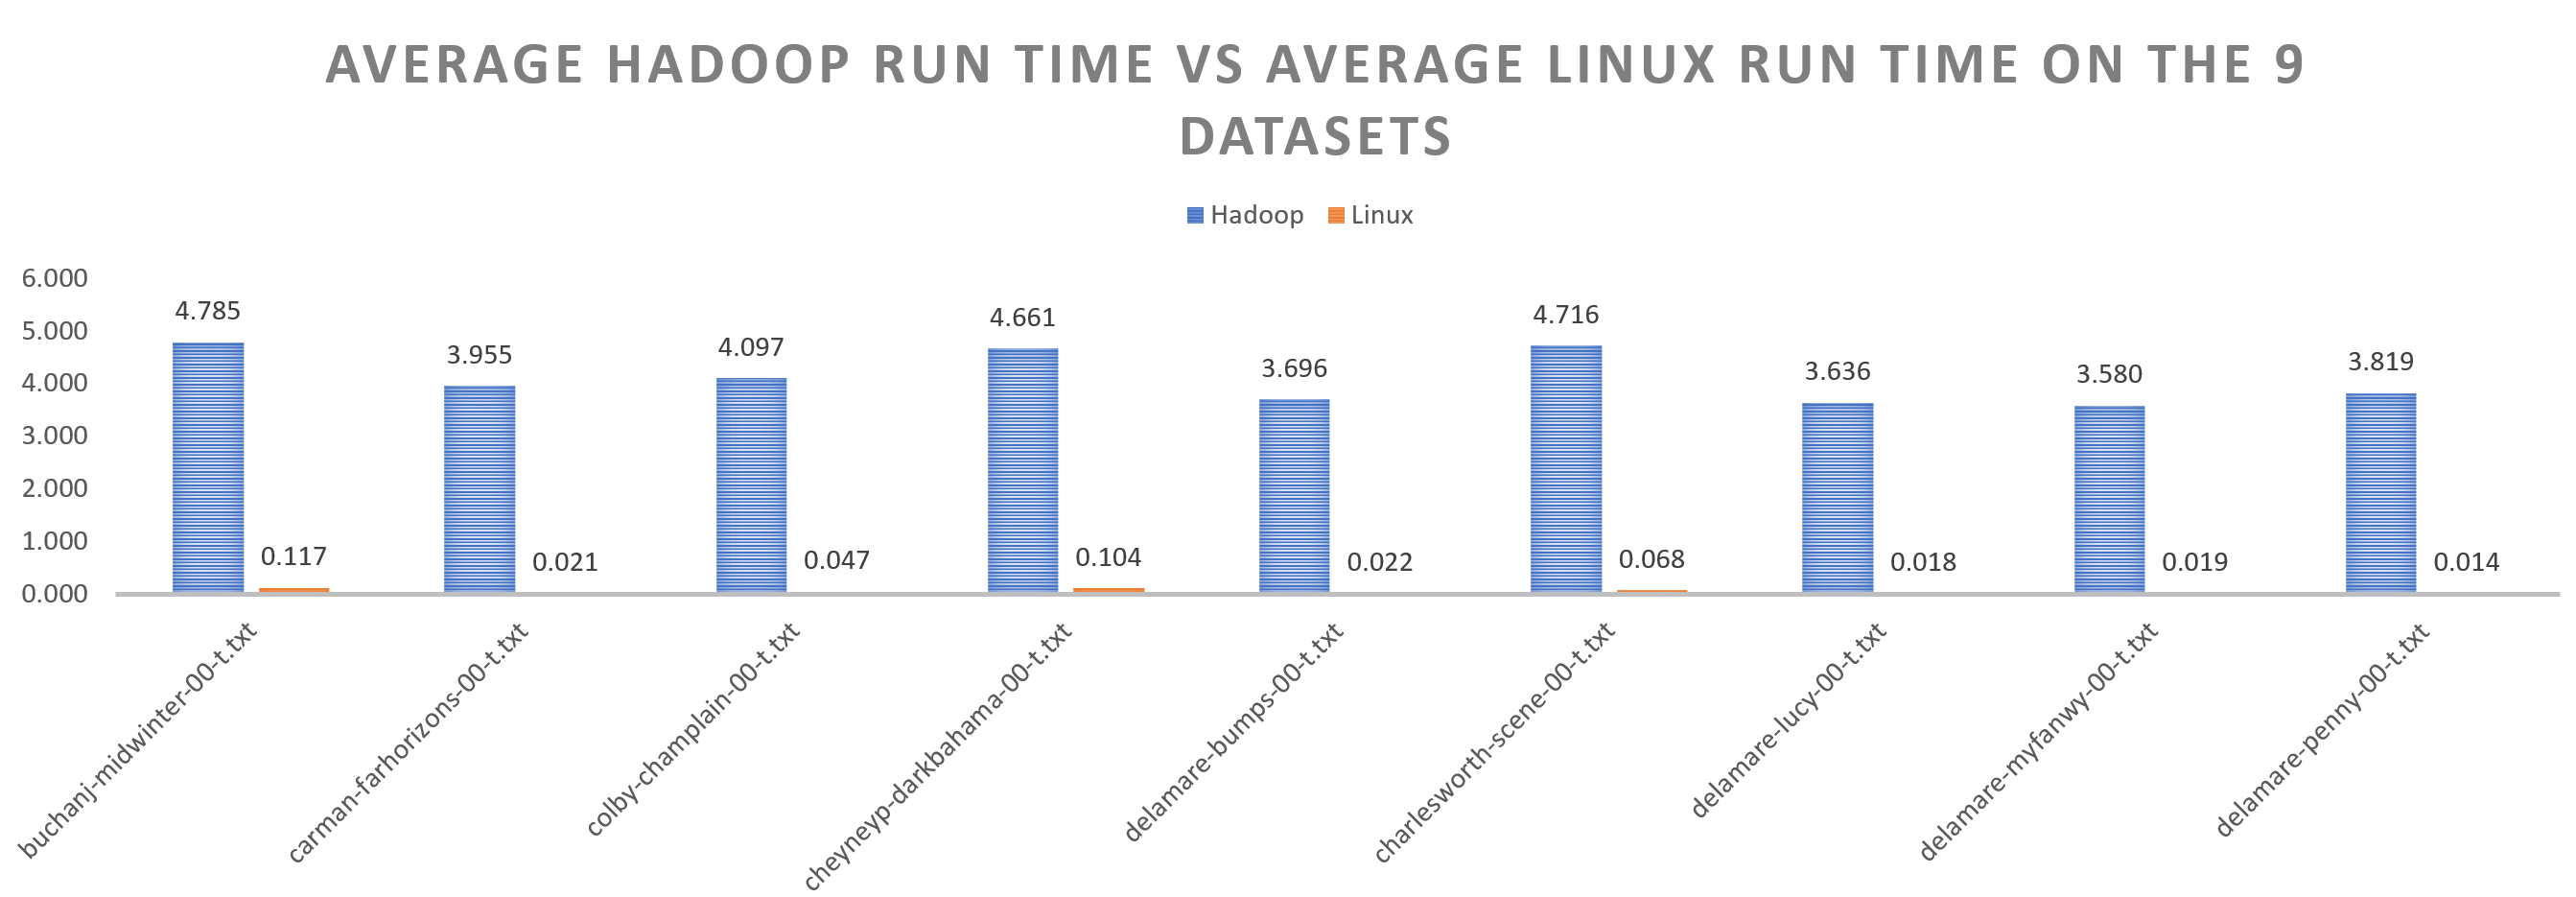
\includegraphics[width=140mm, height=70mm, scale=1.0]{images/Hadoop_vs_Linux_graph.PNG}
    \caption{Result of Hadoop vs. Linux runtime}
    \label{fig:fig4}
\end{figure}

\newpage

\section{Performance comparison of Hadoop vs. Spark on Azure}
\noindent Using the same Azur VM used previously, we used the same method that was used for Hadoop vs. Linux. As such, to properly evaluate both Hadoop and Spark, we ran the WordCount with the \textit{time} command  3 times on each dataset for both. For the spark implementation, we used a python code which known as \textit{SparkWordCount.py}. \\


\noindent On the hand, the command used for Hadoop began with “time hadoop ...”, whereas that with Spark began with “time spark-submit ...”. This information is presented in more detail in our \textit{readme.md} file.

\begin{figure}[H]
    \centering
    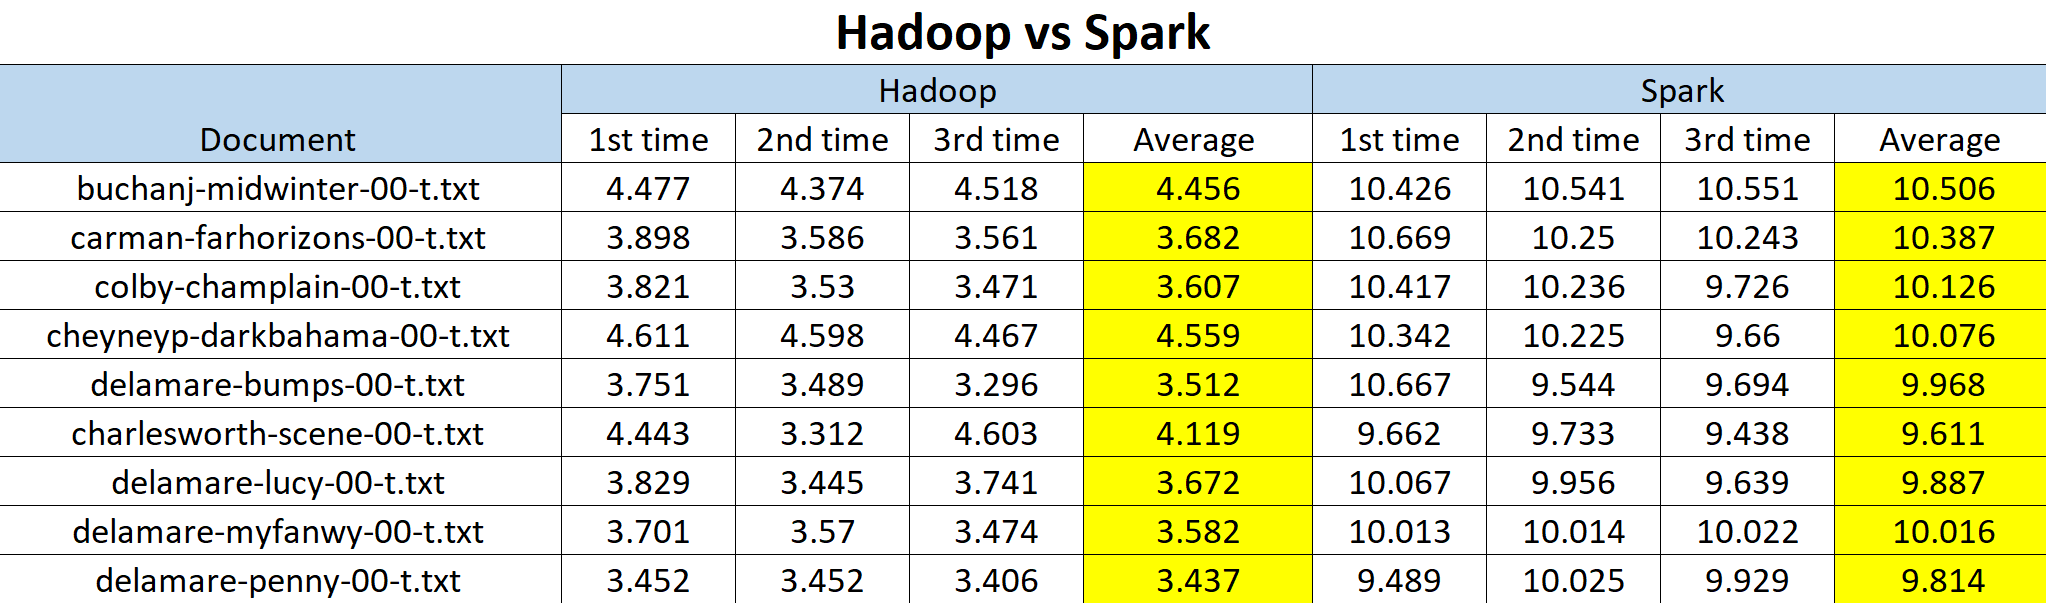
\includegraphics[width=140mm, height=70mm]{images/Hadoop_vs_Spark_table.PNG}
    \caption{Average run time of Hadoop vs. Spark on each dataset}
    \label{fig:fig5}
\end{figure}

\newpage

\subsection{Results}
\noindent Figure~\ref{fig:fig5} depicts the comparison of the consumption time between Hadoop and Spark on each document. Also, for simplicity again, we created a bar chart (Figure\ref{fig:fig6}) that shows the difference in average times between Hadoop and Spark software (all times are in the second unit). It is obvious amongst all datasets Spark took more time for the word counting application in comparison to the Hadoop software. In large datasets, Spark outperforms Hadoop due to the Apache Spark process and parallelization strategy. However, the situation in our assignment is different. We think this problem was due to the different steps of initialisation that Spark needs to set up before beginning to its process. But we have to mention that, Spark supports memory facility but Hadoop does not have this feature. 

\begin{figure}[h]
    \centering
    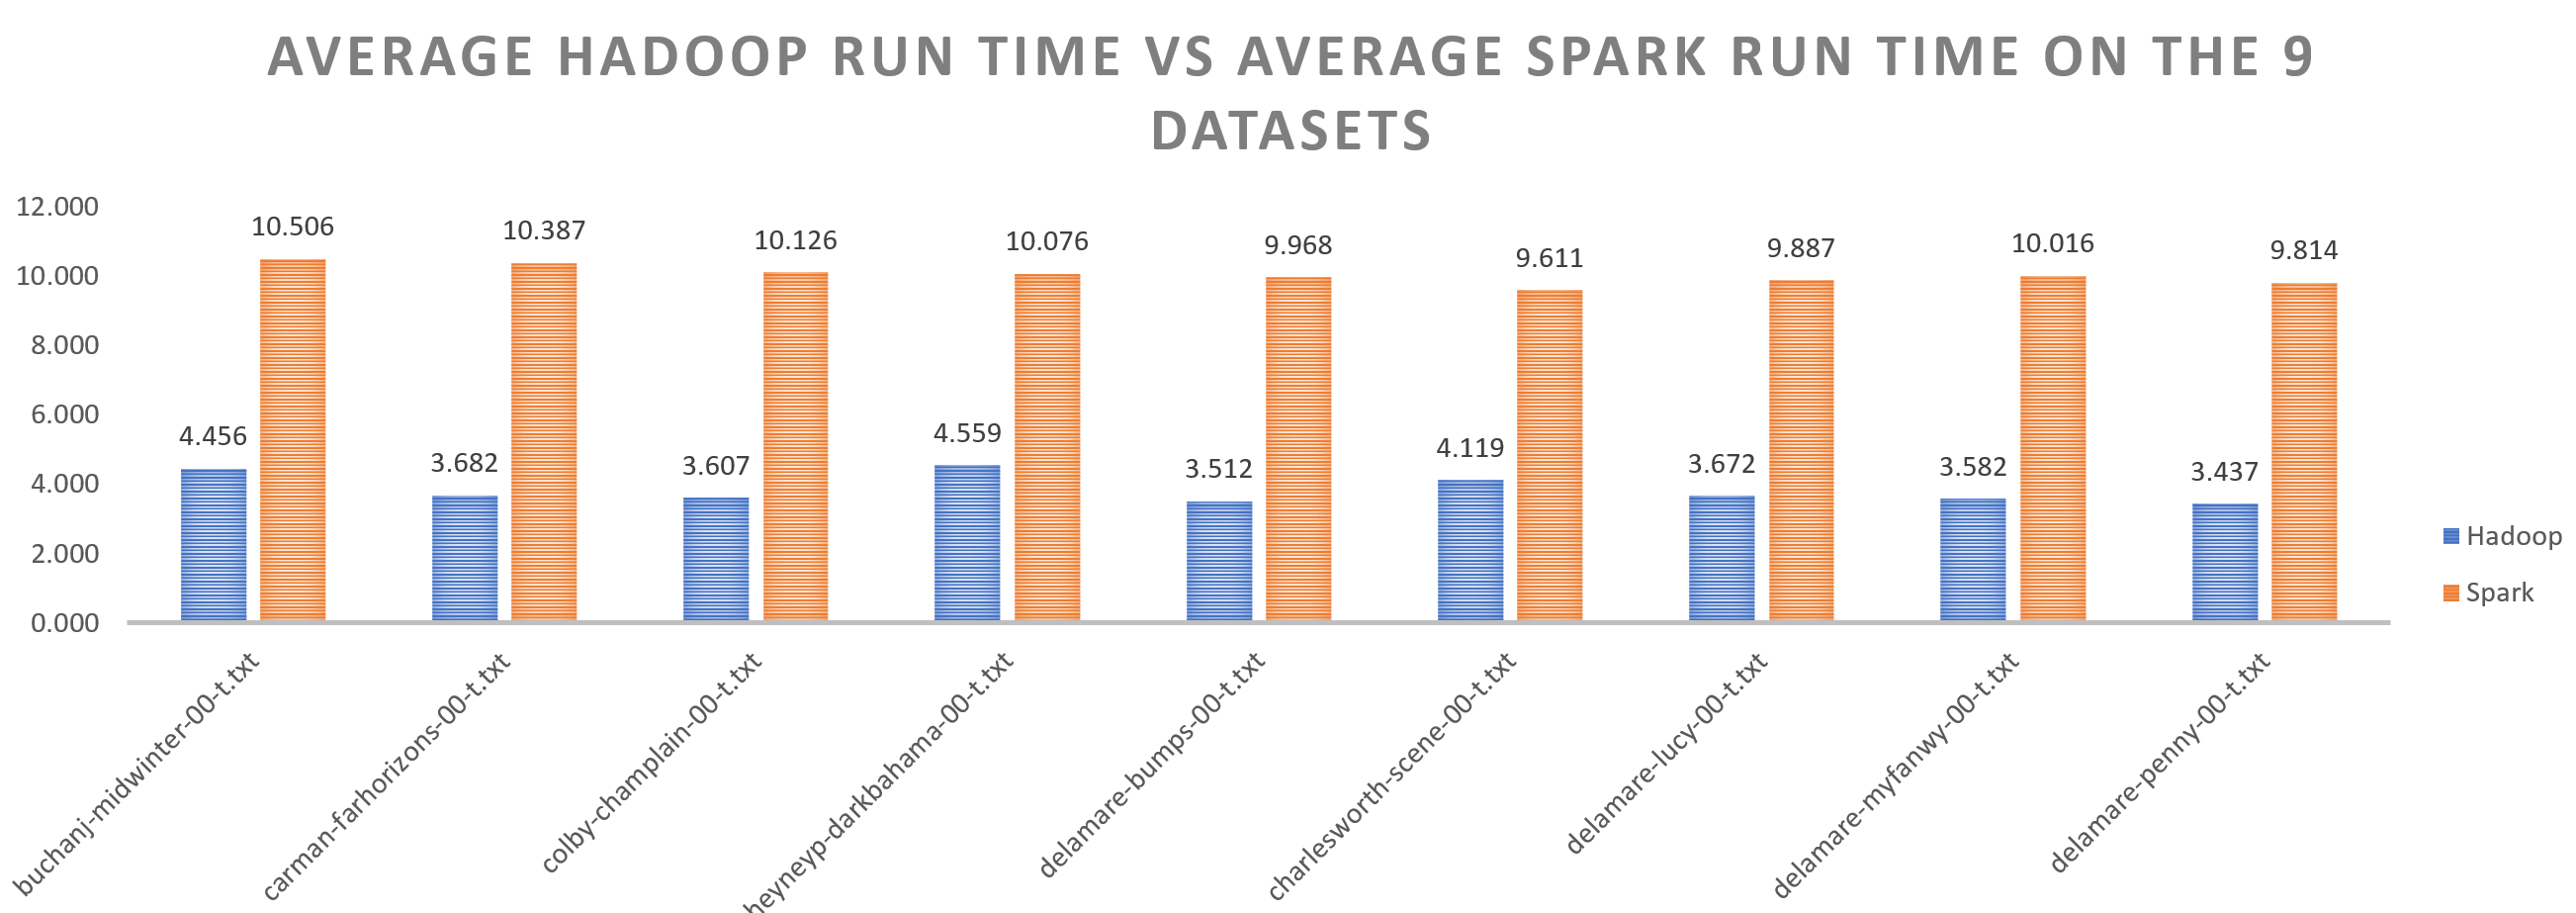
\includegraphics[width=140mm, height=70mm, scale=1.0]{images/Hadoop_vs_Spark_graph.PNG}
    \caption{Result of Hadoop vs. Spark on each dataset}
    \label{fig:fig6}
\end{figure}

\newpage

\section{People you might know problem}

In the last part of the assignment, we want to implement a simple social network friendship recommendation system. The system should suggest the right persons for each \textit{user id}. In this case, our input is a list of users and their associated list of friends, and then we recommend to each user a list of people they might know according to their mutual friends. This could be something similar to the "suggested friends" section when you browse your Facebook feed. In the next section, we discussed a strategy we utilized for the Map and Reduce functions. 

\subsection{MapReduce and algorithm}
\noindent The MapReduce model works based on the key-value approach. Keys are unique, and in this problem, are User IDs. Also, values are the list of User IDs of friends that each user has. \\

\noindent Through that, in the mapping process, we will create a key and value. key contains the User ID, and the value is a list that has potential new friends they are not already friends with, as long as they have at least one friend in common. For creating this list, we eliminated User IDs that have mutual friends with the key, in advance. \\

\noindent In the reducer function, we just focused on the frequency of User IDs in the value part for each key and returns ten recommenders for each User ID.

\newpage 

\subsection{Results}

The below table shows the outcome of our recommender system for each User ID. 

\begin{table}[ht]
    \centering
    \resizebox{12cm}{!}{%
    \begin{tabular}{||c|c||} \hline\hline
       \textbf{User ID}& \textbf{Suggestions} \\\hline
        924 & 439,2409,6995,11860,15416,43748,45881\\\hline
        8941 & 8943,8944,8940\\\hline
        8942 & 8939,8940,8943,8944 \\\hline
        9019 & 9022,317,9023\\\hline
        9020 & 9021,9016,9017,9022,317,9023 \\\hline
        9021 & 9020,9016,9017,9022,317,9023 \\\hline
        9022 & 9019,9020,9021,317,9016,9017,9023 \\\hline
        9990 & 13134,13478,13877,34299,34485,34642,37941 \\\hline
        9992& 9987,9989,35667,9991 \\\hline
        9993& 9991,13134,13478,13877,34299,34485,34642,37941 \\\hline\hline
    \end{tabular}
     }
    \caption{FRIEND SUGGESTIONS}
    \label{tbl:friend_suggestions}
\end{table}

\newpage

\section{Github repository}
\noindent The following public GitHub repository  includes all the files that we used. All codes have comments in themselves and in the \textit{readme.md} file, we precisely explain each step we took for our implementations.

\paragraph{Link:} https://github.com/ghadesi/LOG8415---Advanced-Concepts-in-Cloud-Computing/tree/main/Assignment2
      
      
\newpage

\section{Bibliography}

\begin{enumerate}
    \item Apache spark. http://spark.apache.org.
    \item Apache spark examples. http://spark.apache.org/examples.html. Ac
    \item Hadoop tutorial. http://dzone.com/articles/getting-hadoop-and-running.
    \item Mapreduce tutorial. https://hadoop.apache.org/docs/r1.2.1/mapred-tutorial.html.
\end{enumerate}

\end{document}